% Definierte Informationen

\newcommand{\scrartclScrreprt}{scrartcl}
\newcommand{\trauthorB}{Philipp Riedel}

\newcommand{\trauthorA}{Armin Stocklin}

\newcommand{\trprof}{Prof. Dr. A. Müller}
\newcommand{\trfachgebiet}{Mathematisches Seminar}
\newcommand{\trfakultaet}{Elektrotechnik}
\newcommand{\trdate}{\today}

\newcommand{\titleinfo}{Lichtbrechung als Optimierungsproblem}
\newcommand{\authorinfo}{\trauthorA, \trauthorB}


%!TEX TS-program = pdflatex
\documentclass[numbers=noenddot,abstracton]{\scrartclScrreprt}

\usepackage[numbers]{natbib}
\usepackage[utf8x]{inputenc}
\usepackage[T1]{fontenc}
\usepackage{lmodern}
\usepackage{layout}
\setlength{\parindent}{0em}

\renewcommand{\baselinestretch}{1.2}
\renewcommand{\arraystretch}{1}

\let\oldmarginpar\marginpar
\renewcommand{\marginpar}[1]{\-\oldmarginpar[\raggedleft\scriptsize\hspace{0pt}#1]%
{\raggedright\footnotesize #1}}

%Damit \today ein Deutsch Formatiertes Datum zurueckgibt.  
\usepackage[ngerman, num, orig]{isodate}
\usepackage[ngerman]{babel}   

\monthyearsepgerman{\,}{\,} 

\usepackage{amssymb,amsmath,fancybox,graphicx,wrapfig,color,lastpage,fancyhdr,verbatim,epstopdf,a4wide}
\usepackage{paralist}	%aufzählungen in Tabelle machen

\usepackage{setspace}
\usepackage{epsfig}
\usepackage{supertabular}{\tiny }
\usepackage[font=small,labelfont=bf]{caption}
\usepackage{subcaption}
\usepackage{footnote}
\usepackage{float}
\usepackage{multirow}
\usepackage{etex}
\usepackage{pdfpages}
\usepackage{color} 
\usepackage{placeins} 
\usepackage{booktabs}


\usepackage[makeroom]{cancel}
\usepackage{array}
\usepackage{trfsigns}
\usepackage{textcomp}


% Kompaktes Itemize
\usepackage{enumitem}
\newlist{compactitemize}{itemize}{1}
\setlist[compactitemize]{label=\textbullet, nosep, leftmargin=10pt}


\usepackage{tikz}
\usetikzlibrary{shapes}
\usepackage{pgfplots}
\pgfplotsset{every axis plot/.style={line width=1pt}}
\pgfset{number format/1000 sep={}}
\pgfplotsset{tick label style={/pgf/number format/fixed}}
\pgfplotsset{scaled ticks=false}
\pgfplotsset{compat=newest}


\usepackage[hyphens]{url}	%URL handling und darstellung
\urlstyle{tt}

\usepackage[pdftitle={\titleinfo},
						pdfauthor={\authorinfo},
						pdfcreator={TeXStudio, LaTeX with hyperref},
						plainpages=false,
						pdfpagelabels,
						colorlinks,
						linkcolor=black,
						filecolor=black,
						citecolor=black,
						urlcolor=black]{hyperref}

\usepackage{tabularx}

\renewcommand{\captionfont}{\scriptsize\slshape}




\newcommand{\texttodo}[1]{\textcolor{red}{Todo: #1}}
\setlength{\unitlength}{1mm}

\setcounter{secnumdepth}{3}
\setcounter{tocdepth}{3}
	
%Abbildungsnumerierung anhand Kapitel
\renewcommand{\thefigure}{\arabic{section}.\arabic{figure}}
\makeatletter \@addtoreset{figure}{section} \makeatother

%%%%%%%%%%%%%%%%%%%%%%%%%%%%%%%%%%%%%%%%%%%%%%%%%%%%%%%%%%%%%%%%
% Begin define headings
%%%%%%%%%%%%%%%%%%%%%%%%%%%%%%%%%%%%%%%%%%%%%%%%%%%%%%%%%%%%%%%%
%\renewcommand{\headrulewidth}{0.4pt}
%\renewcommand{\footrulewidth}{0.4pt}

\lhead[\scriptsize\nouppercase{\leftmark}]{}%\textbf{\titleinfo}}
\chead[]{}
\rhead[]{\scriptsize\nouppercase{\leftmark}}%\textbf{\titleinfo}]{}

\lfoot[\scriptsize\thepage]{\scriptsize{}}
\cfoot[]{}
\rfoot[\scriptsize{}]{\scriptsize\thepage}

\AtBeginDocument{\numberwithin{equation}{section}} %Damit Gleichungen mit Section Nummer beginnen
\AtBeginDocument{\numberwithin{figure}{section}}
\AtBeginDocument{\numberwithin{table}{section}}




% referenzen definitionen
\newcommand{\figref}[1]{Abbildung~\ref{#1}}
\renewcommand{\eqref}[1]{Gleichung~\ref{#1}}
\newcommand{\tabref}[1]{Tabelle~\ref{#1}}
\renewcommand{\pageref}[1]{Seite~\ref{#1}}
\newcommand{\chapref}[1]{Kapitel~\ref{#1}~(\nameref{#1})}
\newcommand{\secref}[1]{Abschnitt~\ref{#1}}
\newtheorem{postulat}{Postulat}


% Definitionen von Herr Müller 

\newtheorem{satz}{Satz}
\newtheorem{hilfssatz}{Hilfssatz}
\newtheorem{definition}{Definition}
\newtheorem{annahme}{Annahme}




% Möglichst keine Ergänzungen hier, sondern in header.tex
\begin{document} 
 

% Römische Nummerierung für Sonderseiten, wie Verzeichnisse und Anhang
\pagenumbering{Roman}

% Titelblatt
\thispagestyle{empty}
\begin{center}
\begin{huge}
	\titleinfo
\end{huge}
\vfill
\begin{large}
\begin{tabular}{l p{0.5cm} l} 
  Fachgebiet & & \trfachgebiet \\ \vspace{0.2cm}
  Betreuung der Arbeit  & & \trprof \\   \vspace{0.2cm}
  Studiengang & & \trfakultaet \\ \vspace{0.2cm}
  Vorgelegt von & & \trauthorA $ $ und \trauthorB
\end{tabular}
\end{large}
\end{center}


% Inhaltsverzeichnis
\newpage
\setcounter{tocdepth}{1}
\tableofcontents

% Nummerierung von roemisch auf arabisch umschalten und roemische
% zwischenspeichern
\newpage
\newcounter{roemisch}
\setcounter{roemisch}{\value{page}}
\pagenumbering{arabic}


%\section{Aufgabenstellung}

\subsection{Aufgabe}
Das Licht nimmt immer den kürzesten Weg. Die Lichtgeschwindigkeit
h"angt von der optischen Dichte des Materials ab. Wie wird ein Lichtstrahl gekr"ummt, wenn die optische Dichte nicht konstant ist?

Die Natur regelt die Ausbreitung des Lichtes mit einem Minimumprinzip. Zeigen Sie, wie man aus diesem Minimumprinzip für die Ausbreitung von Lichtstrahlen zum Beispiel in einer Fata Morgana eine Differentialgleichung ableiten kann. Und auch das Brechungsgesetz von Snellius folgt aus diesem Optimumprinzip.

\section{Einleitung}
Wie in den vorangegangen Kapitel oft gesehen, stehen für Optimierungsprobleme verschiedene Programme wie z.B. der Symplex Algorithmus zur Verfügung. Dabei wird ein Maxima oder Minima gesucht. Bei der Variationsrechnung wird, wie in \chapref{chapter-variationsrechnung} beschrieben, eine Funktion gesucht welche, das Optimierungsproblem löst. Für die Variationsrechnung steht anstelle eines mathematischen Programms die Euler-Lagrange-Gleichung zur Verfügung. Wie nützlich und mächtig sie ist, soll anhand von Beispielen in folgenden Seiten etwas aufgezeigt werden.

\section{Einleitende Theorie, Fermatsches Prinzip}

Im Jahre 1660 fand Pierre de Fermat, ein Französischer Mathematiker, dass  nach ihm benannte, Fermatsche Prinzip heraus. 
Dieses lautet wie folgt \cite{DefinitionFermat}:

\begin{postulat}
	Der Weg, den das Licht nimmt, 
	um von einem Punkt zu einem anderen zu gelangen, 
	ist stets so, dass die benötigte Zeit minimal ist.
	\index{Fermatsches Prinzip 1}
\end{postulat}

Die \eqref{fermat} zeigt das Fermatsche Prinzip bei einem Brechungsindex $n$, 
der Lichtgeschwindigkeit $c$, dem Weg $s$ und dem Ort $r$ Die Zeit muss minimal sein.

\begin{align}
	t= \int\limits_{s_1}^{s_2} \frac{n(r)}{c} ds = \frac{1}{c} \int\limits_{s_1}^{s_2} n(r) ds
	\label{fermat}
\end{align}


Wenn die Zeit minimal ist, wird bei kleinen Abweichungen vom Weg die Zeit nicht viel grösser. 
Deshalb kann die oben stehende Definition auch wie folgt geschrieben werden\cite{Definition}.

\begin{postulat}
Der Weg, den das Licht nimmt,  um von einem Punkt zu einem anderen zu gelangen, 
ist stets so, dass die Zeit, die das Licht benötigt, invariant gegen kleine Änderungen des Weges ist.
\index{Fermatsches Prinzip 2}
\end{postulat}

\subsection{Formulierung mit dem optischen Weg}
Der optische Weg $L$  eines Pfades $s$ kann in einem homogenen Material 
mit dem Brechungsindex $n$ als Produkt von $n$ und $s$ berechnet werden.
Bei einem inhomogenen Material ergibt sich für den optischen Pfad die allgemeine \eqref{optischweg}.
\begin{align}
	L(s) = \int\limits_{s_1}^{s_2} n(r) \,\mathrm d\vec s 
	\label{optischweg}
\end{align}

Da der zurückgelegte Weg des Lichtstrahles direkt proportional zur Zeit ist, $s = c \cdot t$,
und das Licht sich in optisch dichteren Materialien langsamer bewegt,
kann das Fermatsche Gesetz umformuliert werden\cite{Definition}. 


\begin{postulat}
Der Weg, den das Licht nimmt, um von einem Punkt zu einem anderen zu gelangen, ist stets so, dass der optische Weg minimal ist.
\index{Fermatsches Prinzip 2}
\end{postulat}

\subsection{Erklärung}
Viele Leute haben ein Problem mit dem Fermatschen Prinzip. 
Der Grund ist ganz einfach. 
Bei der ``klassischen'' Strahlenoptik geht das Licht einen bestimmten Weg, 
sieht einen Spiegel oder eine Oberfläche, bricht sich dort nach einem 
physikalischen Gesetz und geht dann weiter.
Der philosophische Ansatz vom Fermatschen Prinzip ist anders. 
Es wird davon ausgegangen, dass das Licht, bevor es einen Weg einschlägt, 
weiss wohin es muss. Es weiss, wo ein Spiegel oder eine Oberfläche kommt und 
nimmt dem entsprechend von Anfang an den Weg mit der kürzesten Zeit.
Aber woher weiss das Licht, dass sein eingeschlagener Weg der korrekte ist?
Kann man davon ausgehen, dass es die nähere Umgebung anschaut und diese Vergleicht?
Ja, genau davon kann man ausgehen. Eine mögliche Erklärung mit Hilfe von Elektromagnetischen Wellen ist,
dass sich das Licht in alle Richtungen ausbreitet. 
Jedoch interferieren die meisten dieser Wellen destruktiv, 
ausser die Welle, welche den Weg mit der kürzester Zeit genommen hat, wird nicht ausgelöscht.

\section{Rechnung an einem Konkreten Beispiels}

\subsection{Brechungsgesetz von Snellius \label{brechungsgesetz}}
\cite{Wikipedia} Aus dem Fermatschen Prinzip lässt sich das Brechungsgesetz von Snellius herleiten.
Das Licht legt den Weg vom Startpunkt $P_0$ über den Brechungspunkt $P_1$ 
nach dem Endpunkt $P_2$ zurück, siehe \figref{Ab:brechung}.
\begin{figure}[H]
	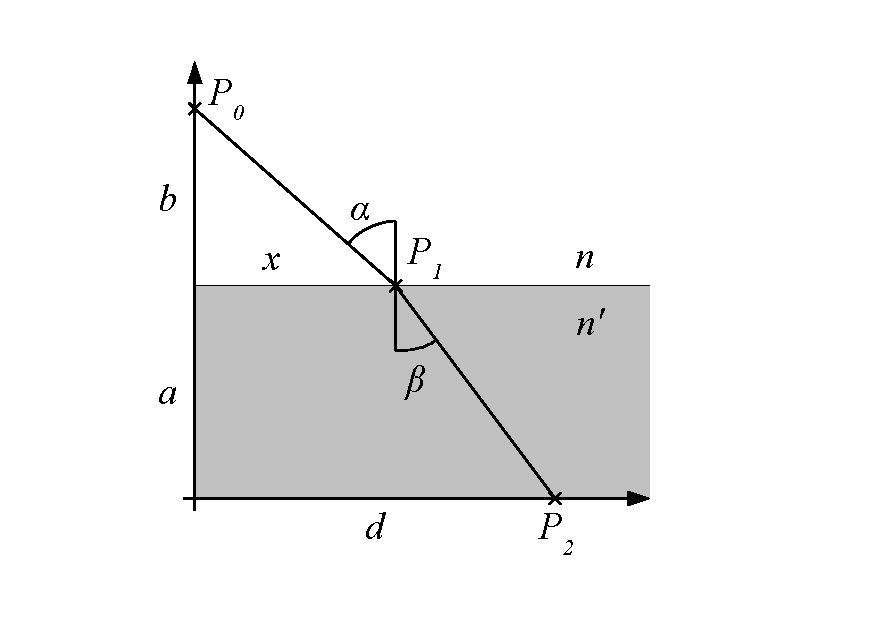
\includegraphics[width=0.8\textwidth]{./picture/Brechung.pdf}
	\caption{Skizze des Brechungsgesetzes von Snellius}
	\label{Ab:brechung}
\end{figure}

Dadurch kann die zurückgelegte Zeit berechnet werden (\eqref{snelliusT}).
\begin{align}
t(x) = t_1 + t_2 = \frac{s_1}{c_1} + \frac{s_2}{c_2} = \frac{|P_1 - P_0|}{c_1} + \frac{|P_2 - P_1|}{c_2} \notag \\
= \frac{\sqrt{a^2 + x^2}}{c_1} + \frac{\sqrt{(d-x)^2 + b^2}}{c_2} \label{snelliusT}
\end{align}

Wird diese Funktion nach $dx$ abgeleitet und gleich Null gesetzt wird die Extremastelle von $t$ gefunden (\eqref{snelliusDx}).
\begin{equation}
	\frac{dt}{dx} = \frac{2 \cdot x}{2 \cdot c_1 \cdot \sqrt{a^2 + x^2}} + \frac{-2 \cdot (d-x)}{2 \cdot c_2 \cdot \sqrt{(d-x)^2 + b^2}} =
	\frac{x}{c_1 \cdot \sqrt{a^2 + x^2}} - \frac{(d-x)}{c_2 \cdot \sqrt{(d-x)^2 + b^2}} = 0 \label{snelliusDx}\\
\end{equation}

Eine weitere Ableitung und einsetzen von $x_0$ welches beim berechnen von (\eqref{snelliusDx}) gefunden wird zeigt ob ein lokales Maxima oder Minima vorliegt.
\begin{align}
\text{mit} c_2=2 \cdot c_1 \qquad a=1 \qquad b=2a \qquad d=1 \textbf{ist} x_0 = 0.190898 \notag \\
\frac{dt}{d^2x}=\frac{1}{c2 \sqrt{b^2 + (d - x)^2}} - \frac{(d - x)^2 }{c2 (b^2 + (d - x)^2)^(3/2)} \notag \\
- \frac{x^2}{c1 (a^2 + x^2)^(3/2)} + \frac{1}{c1 \sqrt{1^2 + x^2}} = y  \notag \\
y =\frac{1.14688}{c1} > 0
\end{align}
$x_0$ ist lokales Minima, da es auch der einzige Kandidat für eine Extremastelle ist, ist es auch ein globales Minimum.



Aus \figref{Ab:brechung} ist gut ersichtlich das die Substitutionen \ref{substitution1} und \ref{substitution2} durchgeführt werden können,

\begin{align}
	\sin(\alpha) = \frac{x}{\cdot \sqrt{a^2 + x^2}}  \label{substitution1}\\
	\sin(\beta) = \frac{d-x}{\sqrt{(d -x)^2 + b^2}} \label{substitution2}
\end{align}

Nach etwas umformen ergibt sich, das Verhältnis der Winkel $\alpha \ \text{und} \ \beta$ gemäss (\eqref{snellius}).

\begin{equation}
	0 = \frac{\sin(\alpha)}{c_1} - \frac{\sin(\beta)}{c_2} \Leftrightarrow\frac{c_2}{c_1} = \frac{\sin(\beta)}{\sin(\alpha)}
	\label{snellius}
\end{equation}


\subsection{Reflexionsgesetz}
\cite{Wikipedia} Auf gleiche weise wie das das Brechungsesetz aus dem Fermatschen Prinzip hergeleitet wird, 
lässt sich daraus auch das Reflexionsgesetz ableiten.
Das Licht legt den Weg vom Startpunkt $P_0$ über den Spiegelpunkt $P_1$ 
nach dem Endpunkt $P_2$ zurück. Dadurch kann die zurückgelegte Zeit berechnet werden (\eqref{reflexion}).


\begin{align}
t(x) = t_1 + t_2 = \frac{s_1 + s_2}{c} = \frac{|P_1 - P_0| + |P_2 - P_1|}{c} \notag \\
= \frac{\sqrt{a^2 + x^2} + \sqrt{(d-x)^2 + b^2}}{c} \label{reflexion}
\end{align}

Wenn $t(x)$ nach $dx$ abgeleitet und gleich 0 gesetzt wird ergibt sich die Extremastelle  von $t$ (\eqref{reflexionDx}). Auf den Beweis das es ebenfalls ein Minimum ist wie bei der Reflexion wird hier verzichtet.

\begin{align}
\frac{dt}{dx} = \frac{1}{c} \cdot \frac{2 \cdot x}{2 \cdot \sqrt{a^2 + x^2}} + \frac{-2 \cdot (d-x)}{2 \cdot \sqrt{(d-x)^2 + b^2}} \notag \\
= \frac{x}{ \sqrt{a^2 + x^2}} - \frac{(d-x)}{ \sqrt{(d-x)^2 + b^2}} = 0 \label{reflexionDx}
\end{align}

\begin{figure}[H]
	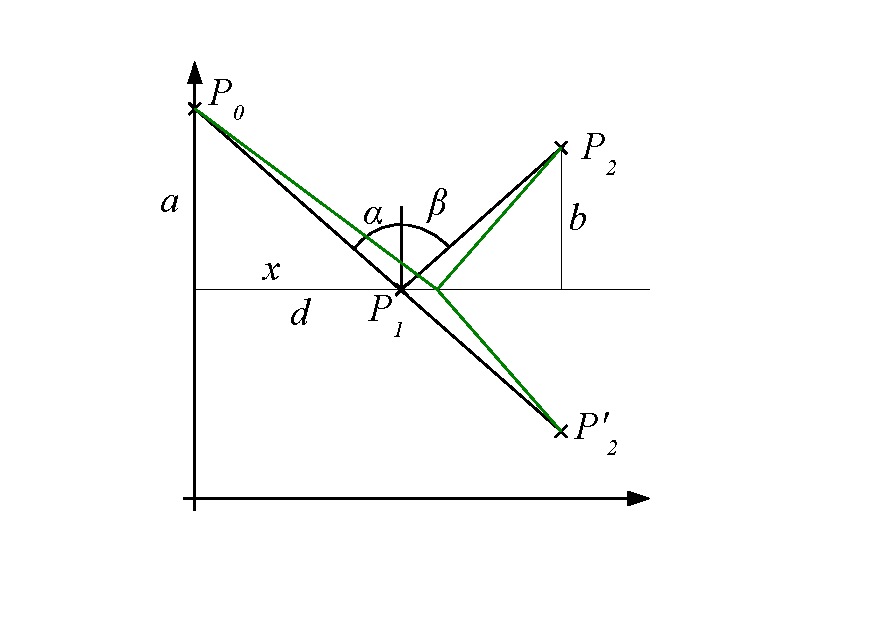
\includegraphics[width=0.8\textwidth]{./picture/Spiegelung.pdf}
	\caption{Skizze des Reflexionsgesetzes}
	\label{Ab:spiegelung}
\end{figure}

In \figref{Ab:spiegelung} ist ersichtlich, dass die Substitutionen \ref{substitution1} und \ref{substitution2} von \secref{brechungsgesetz} auch hier nützlich sind.
Nach etwas umformen ergibt sich, dass Eintritts- und Austrittswinkel gleich sind (\eqref{brechung}).


\begin{equation}
0 = \sin(\alpha) - \sin(\beta) \Leftrightarrow \sin(\beta) = \sin(\alpha) \Leftrightarrow\beta = \alpha
\label{brechung}
\end{equation}

In \figref{Ab:spiegelung} ist ersichtlich, dass die Linie des Startpunktes bis zum 
gespiegelten Endpunkt eine Gerade ist, welche der Funktion des kürzesten Weges entspricht.

\section{Berechnungen mittels Euler-Lagrange Gleichung}
\subsection{Einleitung}
Einige Probleme lassen sich direkt lösen, indem sie in die hergeleitete Euler-Lagrange-Gleichung eingesetzt werden können. Andere Optimierungsprobleme, bei denen eine Funktion gesucht wird, können gelöst werden, indem sie das Prinzip der Variation von der Euler-Lagrange-Gleichung benutzen. Dazu reicht jedoch nicht mehr ein einfaches einsetzen, sondern es muss eine neue Gleichung hergeleitet werden. Die gesuchte Funktion wird dann gefunden, indem für $g(y)$ und $g'(y)$ konkret $y(x)$ und $y'(x)$ eingesetzt wird. Aber dazu später noch mehr.

\subsection{Beschreibung einer Fata Morgana}
\cite{fataEinleitung}
Bei der physikalischen Betrachtung der Lichtausbreitung geht man davon aus, dass sich Licht in
geradlinig verlaufenden Strahlen fortpflanzt. Das Auge erwartet das Objekt, von dem die Lichtstrahlen
kommen, in rückwärtiger geradliniger Verlängerung der Richtung, welche das Licht beim eintreffen in das Auge besitzt.

Wenn das Licht ein Medium, z.B. mit unterschiedlichen Brechungsindizes durchquert, ändert es seine Richtung wie in \secref{brechungsgesetz} gezeigt. Dies erklärt z.B. die verkürzten Beinen im Schwimmbad.
Eine kompliziertere Situation liegt vor, wenn der Brechungsindex des durch-strahlten Mediums kontinuierlich variiert. 
Dies ist der Fall, wenn die Luft in der Nähe eines stark aufgeheizten Untergrundes erwärmt
wird und infolge der dadurch bewirkten Dichteänderung einen räumlichen variierenden Brechungsindex annimmt. 
Das Licht ändert stetig seine Richtung, dass führt zu Phänomenen wie Luftspiegelungen von Autolichtern oder einer Fata Morgana, an heißen Tagen.

Eintritt in das Auge besitzt. In \figref{Ab:fataEinleitung} wird die Wahrnehmung des Auges und eine Richtungsänderung des Lichtes gezeigt.

\begin{figure}[H]
\begin{center}
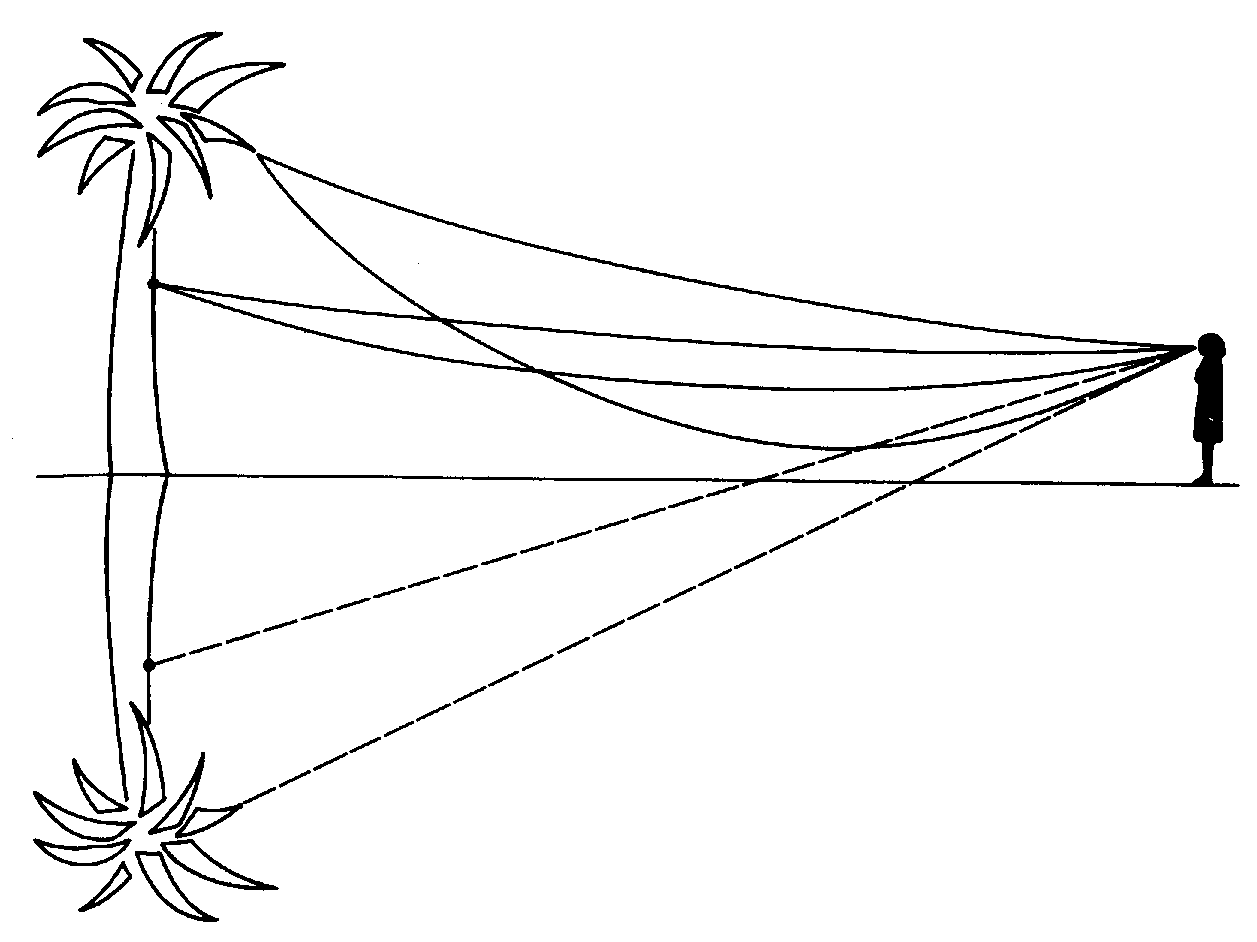
\includegraphics[width=0.5\textwidth]{./picture/FataEinleitung.png}
	\caption{Das Auge interpretiert, dass die Lichtstrahlen mit veränderter Richtung aus der tangentialen Verlängerung kommen und sieht dort das Bild}
	\label{Ab:fataEinleitung}
\end{center}	
\end{figure}


\subsection{Untersuchung der Krümmungs-Eigenschaften bei einer räumlichen Dichteänderung \label{sec:Krümmung}}

Bei einer Fata Morgana hat die Luft eine optische Dichte von $n(x,y)$. 
Dabei bewegt sich das Licht mit der Geschwindigkeit $c/n(x,y)$. 
Die benötigte Zeit, damit das Licht vom Punkt $(x_0, y_0)$ nach $(x_1, y_1)$ braucht,
kann mit dem Kurvenintegral berechnet werden (\eqref{funktionTy}).

\begin{equation}
	T(y) = \int \limits_{x_0}^{x_1} \frac{n(x,y)}{c} \sqrt{1 + y'(x)^2} dx
	\label{funktionTy}
\end{equation}

Wie es bei einem heissen Tag auf einer Strasse oder in einer Wüste zutrifft,
nehmen wir zuerst nur einmal an, dass die optische Dicht nur von $y$ abhängt,
$n(x,y) = g(y)$ und mit zunehmenden $y$ zunimmt.
Dies bedeutet für die Funktion $g(y)$, dass $g(y) > 0$ und $g'(y) > 0 $ ist.

Um dieses Minimalproblem zu lösen, wird die Euler-Lagrange-Gleichung des Variationsproblems aufgestellt (\eqref{krümmung}).

\begin{equation}
	T(y) = \int \limits_{x_0}^{x_1} \frac{g(y)}{c} \sqrt{1 + y'(x)^2} dx = \frac{1}{c} \int \limits_{x_0}^{x_1} g(y) \sqrt{1 + y'(x)^2} dx
	\label{krümmung}
\end{equation}

Der Faktor $\frac{1}{c}$ hat keinen Einfluss auf das Integral und somit auch nicht auf das Variationproblem, deshalb kann er weggelassen werden, um ihn nicht ständig mitschleppen zu müssen.
Es werden nun die Ableitungen der Funktion \ref{funktionRech} gebraucht. Sie sind in \ref{ableitungenLag} aufgeführt.
\begin{equation}
	F(x,y,y') = g(y) \sqrt{1 + y'^2}
	\label{funktionRech}
\end{equation}

\begin{align}
	\frac{\partial F}{\partial y} &= g'(y) \sqrt{1 + y'^2} \notag \\
	\frac{\partial F}{\partial y'} &= g(y) \frac{y'}{\sqrt{1 + y'^2}}
	\label{ableitungenLag}
\end{align}

Für die Euler-Lagrange-Gleichung muss man im zweiten Ausdruck für $y$ und $y'$ die Funktionen $y(x)$ 
sowie $y'(x)$ einsetzen und nach $\frac{d}{dx}$ ableiten, (\eqref{lagrange1}).

\begin{align}
	\frac{d}{dx} \frac{\partial F}{\partial y'} = \frac{d}{dx} (g(y(x)) \frac{y'(x)}{\sqrt{1 + y'(x)^2}}) =
	 \notag \\ g'(y(x)) \frac{y'(x)^2}{\sqrt{1 + y'(x)^2}} + g(y(x)) \frac{y''(x)}{\sqrt{1 + y'(x)^2}} -
	 g'(y(x)) \frac{y'(x)^2 y''(x)}{(1 + y'(x))^\frac{3}{2}} 
	 \label{lagrange1}
\end{align}

Auch im zweiten Term der Euler-Lagrange-Gleichung wird für $y'$ $y'(x)$ eingesetzt. Es ergibt sich \eqref{lagrange2}
\begin{align}
	0 = \frac{d}{dx} \frac{\partial F}{\partial y'} - \frac{\partial F}{\partial y} = 
	g'(y(x)) \frac{y'(x)^2}{\sqrt{1 + y'(x)^2}} + g(y(x)) \frac{y''(x)}{\sqrt{1 + y'(x)^2}} - \notag \\
	g'(y(x)) \frac{y'(x)^2 y''(x)}{(1 + y'(x)^2)^\frac{3}{2}}  - g'(y(x)) \sqrt{1 + y'(x)^2}
	\label{lagrange2}
\end{align}

Da $\sqrt{1 + y'(x)^2} > 0$ und somit nicht gleich Null ist kann die Gleichung mit $\sqrt{1 + y'(x)^2}$  multipliziert werden um einen einfacheren Ausdruck zu bekommen, (\eqref{lagrange3}).

\begin{align}
	0 = g'(y(x)) y'(x)^2 + g(y(x)) y''(x) - g'(y(x)) \frac{y'(x)^2 y''(x)}{1 + y'(x)^2} - g'(y(x)) (1 + y'(x)^2)
	\label{lagrange3}
\end{align}

Auch $g(y(x))$ ist nicht gleich Null, da nach eingangs erfolgter Definition $g(y(x)) > 0$, eine Division mit $g(y(x))$ ist somit zulässig, (\eqref{lagrange4}).

\begin{align}
	\frac{g'(y(x))}{g(y(x))} (1 + y'(x)^2) - \frac{g'(y(x))}{g(y(x))} y'(x)^2 &=  y''(x) - \frac{y'(x)^2 y''(x)}{1 + y'(x)^2} \notag \\
	\frac{g'(y(x))}{g(y(x))} (1 + y'(x)^2 - y'(x)^2) &= \frac{\left(1 + y'(x)^2 \right)y''(x) - y'(x)^2 y''(x)}{1 + y'(x)^2} \notag \\
	\frac{g'(y(x))}{g(y(x))} = \frac{y''(x) + y'(x)^2 y''(x) - y'(x)^2 y''(x)}{1 + y'(x)^2} &= \frac{y''(x)}{1 + y'(x)^2}\notag \\
	\frac{g'(y(x))}{g(y(x))} &= \frac{y''(x)}{1 + y'(x)^2}
	\label{lagrange4}
\end{align}


\eqref{lagrange4} kann jetzt auf ihre Eigenschaften bezüglich der Krümmung untersucht werden. Gemäss den Definitionen von ganz am Anfang ist die linke Seite positiv. 
Der Nenner der rechte Seite ist ebenfalls positiv, daraus resultiert, dass der Zähler der rechten Seite ebenfalls positiv sein muss, (\eqref{krümmungAuswertung}).

\begin{align}
	\frac{g'(y(x))}{g(y(x))} > 0 \qquad \wedge \qquad (1 + y'(x)^2) > 0 \qquad \Rightarrow \qquad y''(x) > 0
	\label{krümmungAuswertung}
\end{align}

Da die zweite Ableitung positiv ist, muss die Funktion des Lichtstrahles konvex sein.
Dies bedeutet, dass der Lichtstrahl sich über dem Boden nach oben biegt, ganz egal wie die Funktion von $g(x)$ aussieht, solange sie monoton steigend ist.
Daraus kann die verallgemeinerte Schlussfolgerung gezogen werden, dass der Lichtstrahl konkav sein muss, wenn die Funktion $g(x)$ monoton fallend ist.
\begin{hilfssatz}
Ein Lichtstrahl wird in einem inhomogenen Medium in Richtung höherer Dichte gekrümmt, verhält sich die Dichteänderung monoton fallend oder steigend, nimmt der Lichtstrahl eine konvexe oder konkave Kurvenform an.
\index{Krümmung von Lichtstrahlen}
\end{hilfssatz}

\subsubsection{Technische Anwendung dieser Erkenntnis}
In einem Lichtwellenleiter wird dieses Phänomen ausgenutzt, indem die untere Seite des Lichtleiters eine monoton steigende
und die obere Seite des Lichtleiters eine monoton fallende Funktion ist. 
Dadurch ist das Licht dann im Leiter ''gefangen'' und kann nicht über einen Rand hinausgehen.

\subsection{Berechnung der Differentialgleichung einer Fata Morgana}

Für die gesuchte Differentialgleichung der Fata Morgana nehmen wir wie bei der Krümung an das die optische Dichtung nur $y$ abhängt. Durch die geringe Krümmung der Erde kann die $x$ Richtung vernachlässigt werden.
$n(x,y) = g(y)$ und mit zunehmenden $y$ zunimmt. Dies bedeutet wie für die Funktion $g(y)$ wie in \secref{sec:Krümmung}, dass $g(y) > 0$ und $g'(y) > 0 $ ist.

Die Euler-Lagrange-Gleichung wird gleich wie in \secref{sec:Krümmung} berechnet. Bei \eqref{lagrange4} wird weiter gerechnet. In (\eqref{diffgleichung1}) werden alle Terme auf die linke Seite genommen.
\begin{align}
	g(y(x)\cdot y''(x)-g'(y(x)\cdot y'(x)^2 - g'(y(x)) =0 
	\label{diffgleichung1}
\end{align}

$g(y(x))$ ist unsere Funktion des Brechungsindex $n(y)$. Mit dieser Substitution ergibt sich differentiationsgleichung (\eqref{diffgleichung2}).
\begin{align}
	n\cdot y''-n'\cdot (y')^2 - n' =0 
	\label{diffgleichung2}
\end{align}

In \secref{sec:Krümmung} war die anfangs definiert worden das die Dichte ab dem Boden richtung $y$ zunimmt weil die Temperatur über dem Boden von dem heissen Untergrund mehr erhitzt ist als in höheren Lagen. Wird jetzt diese Temperaturabnahme als linear angenommen, gilt \eqref{einsetzGl1} und deren Ableitung (\eqref{einsetzGl2}).
\begin{align}
	n(y)&=my+b \label{einsetzGl1} \\
	n'(y)&=m \label{einsetzGl2}
\end{align}

Um die Differentiation Gleichung zu lösen, kann für $y$ eine hyperbolische Funktion gewählt werden (\eqref{hyperFunk}).
\begin{align}
	y&=A\cdot\cosh(Bx+C)+D \label{hyperFunk} \\
	y'&= A\cdot B\cdot sinh(B x + C) \label{hyperFunkDx} \\
	y''&= A\cdot B^2\cdot cosh(B x + C) \label{hyperFunkD2x}
\end{align}


\subsubsection{Eine Beispiel Aufgabe}

Folgende Annahmen gelten:

%\begin{tabularx}{\textwidth}{XX}
%	$y_0=y_1=2 m$ & Augenhöhe und Startpunkt \\
%	$-x_0=x_1 = 200m$ & Temperatur Luft auf Augenhöhe \\
%	$T_A=333.15 K$ & Temperatur des Aspalt \\
%	$T_L=293.15 K$ & Temperatur Luft auf Augenhöhe \\
%	$-x_0=x_1 = 200m$ & Temperatur Luft auf Augenhöhe \\
%\end{tabularx}

\begin{align}
	y_0=y_1=2 m \qquad& Augenhöhe und Startpunkt \\
	-x_0=x_1 = 200m \qquad& Temperatur Luft auf Augenhöhe \\
	T_A=333.15 K \qquad& Temperatur des Aspalt \\
	T_L=293.15 K \qquad& Temperatur Luft auf Augenhöhe \\
	-x_0=x_1 = 200m \qquad& Temperatur Luft auf Augenhöhe \\
\end{align}

Daraus ergeben sich mit \eqref{brechTemp} eine Funktion für den Brechungsindex von Luft in abhängigkeit von Temperatur.
\begin{align}
	n=1+0.000293\frac{T_0}{T}
	\label{brechTemp}
\end{align}
Daraus ergeben sich die werte in \eqref{nParam} für unsere lineare gleichung $n(y)=my+b$
\begin{align}
	y&=y_0=y_1 \notag \\
	b&=n_A=1+0.000293\frac{273.15 K}{333.15 K} = 1.00024 \notag \\
	n_L&=1+0.000293\frac{273.15 K}{293.15 K} = 1.00027 \notag \\
	m&=\frac{\delta n}{y}=\frac{n_L-n_A}{y}=1.64*10^{-5} \notag \\
	n(y)&=my+b=1.64*10^{-5}y +1.00024
	\label{nParam}
\end{align}

Als erstes die allgemeine Form mit einsetzen von $n,n',y',y''$ (\eqref{HauptGl}).
\begin{align}
	(my_0+b)A\cdot B^2\cdot cosh(B x_0 + C)-m (A\cdot B\cdot sinh(B x_0 + C))^2-m &= 0\notag \\
	(my_1+b)A\cdot B^2\cdot cosh(B x_1 + C)-m (A\cdot B\cdot sinh(B x_1 + C))^2-m &=0 \label{HauptGl}
\end{align}

Da wir $y_0$ und $y_1$ gleich haben und $-x_0=x_1$ eine Achsenspieglung und Cosinus Hyperbolicus Funktion eine gerade Funktion ist lässt sich (\eqref{HauptGl}) vereinfachen (\eqref{glvereinfacht}). Dabei wird $C$ weggelassen.
\begin{align}
	(my_0+b)A\cdot B^2\cdot cosh(B x_0 )-m (A\cdot B\cdot sinh(B x_0 ))^2-m &= 0\notag \\
	(my_1+b)A\cdot B^2\cdot cosh(B x_1 )-m (A\cdot B\cdot sinh(B x_1 ))^2-m &=0 \label{glvereinfacht}
\end{align}



% Literaturverzeichnis
\addcontentsline{toc}{section}{Literaturverzeichnis}
%\renewcommand{\refname}{Literaturverzeichnis}
\bibliographystyle{natdin}	%gerplain: [1], geralpha: [Bjar05]
\bibliography{Literatur}


\end{document}


